\section{Case Study: Application of the Framework at Lotaris}

The main business in Lotaris SA is the license management. We develop a solution to manage and provide license management for ISV (Independent software vendor). In our solution, we develop different server side components shown on Fig. \ref{fig:globArchi}. We based our developments on Java technologies and especially Java Enterprise technologies where we use JPA\cite{jpa}.

\begin{figure}[h]
        \centering
        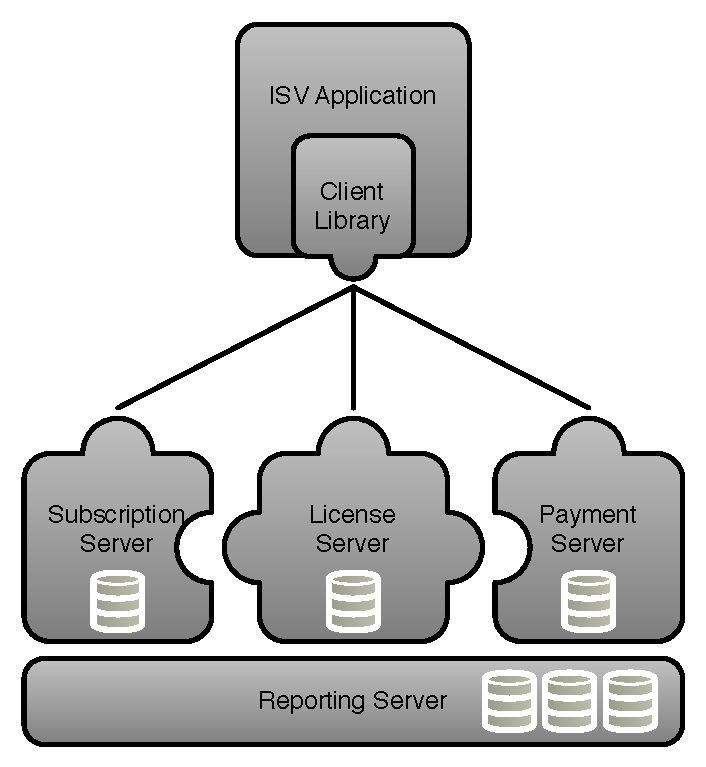
\includegraphics[scale=0.5]{images/archi-glob.pdf}
        \caption{Global architecture}
        \label{fig:globArchi}
\end{figure}

In such context, we use JPA as an ORM that offers an easy way to develop the data binding between the database and the application. As we have started from zero, we have used the ORM from the application to the database. This approach implies some flexibility in terms of developments and relies on the capability of the ORM. We do not need to manipulate directly SQL commands directly due to the mechanism offered by the abstraction of JPA. This is really appreciable but we loose some controls on specific behaviors and performance aspects. We have the possibility to write native SQL but we avoid this solution as much as possible. We tried to write only data access through the API offered by JPA. In other hand, when the configuration is done properly, the database schema is auto-generated and deployed when the application is deployed in the application server. 

Like every great technology, there are several disadvantages like the fact that you do not realize directly that your modification of the code could occur a database change. Adding an attribute to a data model class will produce a new column on the database schema. The code is more easy to change than the database. So, we specially need process to trigger these modifications as we presented in the \autoref{sec:def}.

At Lotaris, we are using SCRUM methodology. This methodology is part of Agile methodologies. We organize our work in sprints of two-three weeks between each release. It means that each sprint we have a new version with potentially database modifications. The Agile methodologies are organized around the possibility to evolve applications to the market needs, to change the user requirements as soon as possible in the development cycle. In general, it always means feature modifications, domain model modifications and so on. These abilities allow mitigating risky modifications and evolving before the application development is too far. One of the main aspect is the fact to build an application as simpler as possible and refactoring only when it is required. Following this way means a lot of modifications that will impact our databases.

Our goal is to keep this methodology for the agile ability. For that, we absolutely need processes and tools to help us in the development cycle. We need to keep easiness of development and fast deployments. We expect everyone is able to write some basic queries (DDL, SQL, ...) or more complex with the help of senior developers. As we discussed in \autoref{sec:def:developer}, each developer is responsible for his modifications and their impacts. It does not mean nobody will help developers to write tricky queries. 

When we started the work on the migrations, we had no clear processes or tools. We started to build iteratively each piece that compose our framework. As we have production imperatives, we had to deal with the schedules and what we could do to improve our migration work. For now, we only deployed in production one of our components with the shared code.

\subsection{Initial deployment of an applciation}

The first deployment of an application is pretty easy. We start from scratch and database schema and data are quite scoped. It is easy to prepare the release based on testing data and infrastructural data. Other required data are quite easy to insert at the beginning. With few SQL scripts, we create the initial stage of an application. The application has no business data and starts its production lifecycle. From this point, the application needs well done migrations each time the application evolves. For these reasons and ones we already discussed, we need to start to think about the migration process. Otherwise, we encounter the same problems that we had when we did our first migrations.

\subsection{Migration pre framework}

When we prepared our migrations, we started to ask us some questions to organize the data migration part. The application did not contain too much model modification that required data migration. It was quite easy to follow modifications and to write the relative migration scripts. At this stage, we already put in place some rules like the separation between queries that could be applied to all environment than the ones that could not be applied on all environments. But all the stuff done at this stage was really handy and specially difficult to handle correctly.

Our experience from these migration were quite awful. We did all by hand and we had no confidence in our migrations. All was done in urgent way with the consequences that could happened. We had done these migrations in pair programming to enhanced the efficiency of the tasks required for the migrations. We had cross-checked our scripts and validated them in a local environments. It was particularly difficult to retrieve the changes and to write the relative scripts. One developer was in charge of the migration. He had to retrieve the modifications and to write the missing scripts with the help of other developers. He had to compare database schemas manually to be sure no modification was missing.

We use Subversion\cite{subversion} as our versioning system. It is a centralized versioning system with a revision numbering system that is incremental. During this first migration, we used the revision number to name our migration script. This trick allows us following the modification by the script file name. We go through all the revisions implied in the migration to analyze and write the migration scripts. The \autoref{fig:StatMig1} shows the information about one of our migrations. The statistics were gathered directly from migration script. We had separated the scripts between our shared component and application component. Each component had its own directory that contains the migration scripts. For the script that must be run only on the specific production environment, we stored them in a specific directory without any structure. We stored the scripts by topics.

\begin{figure}[h]
        \centering
        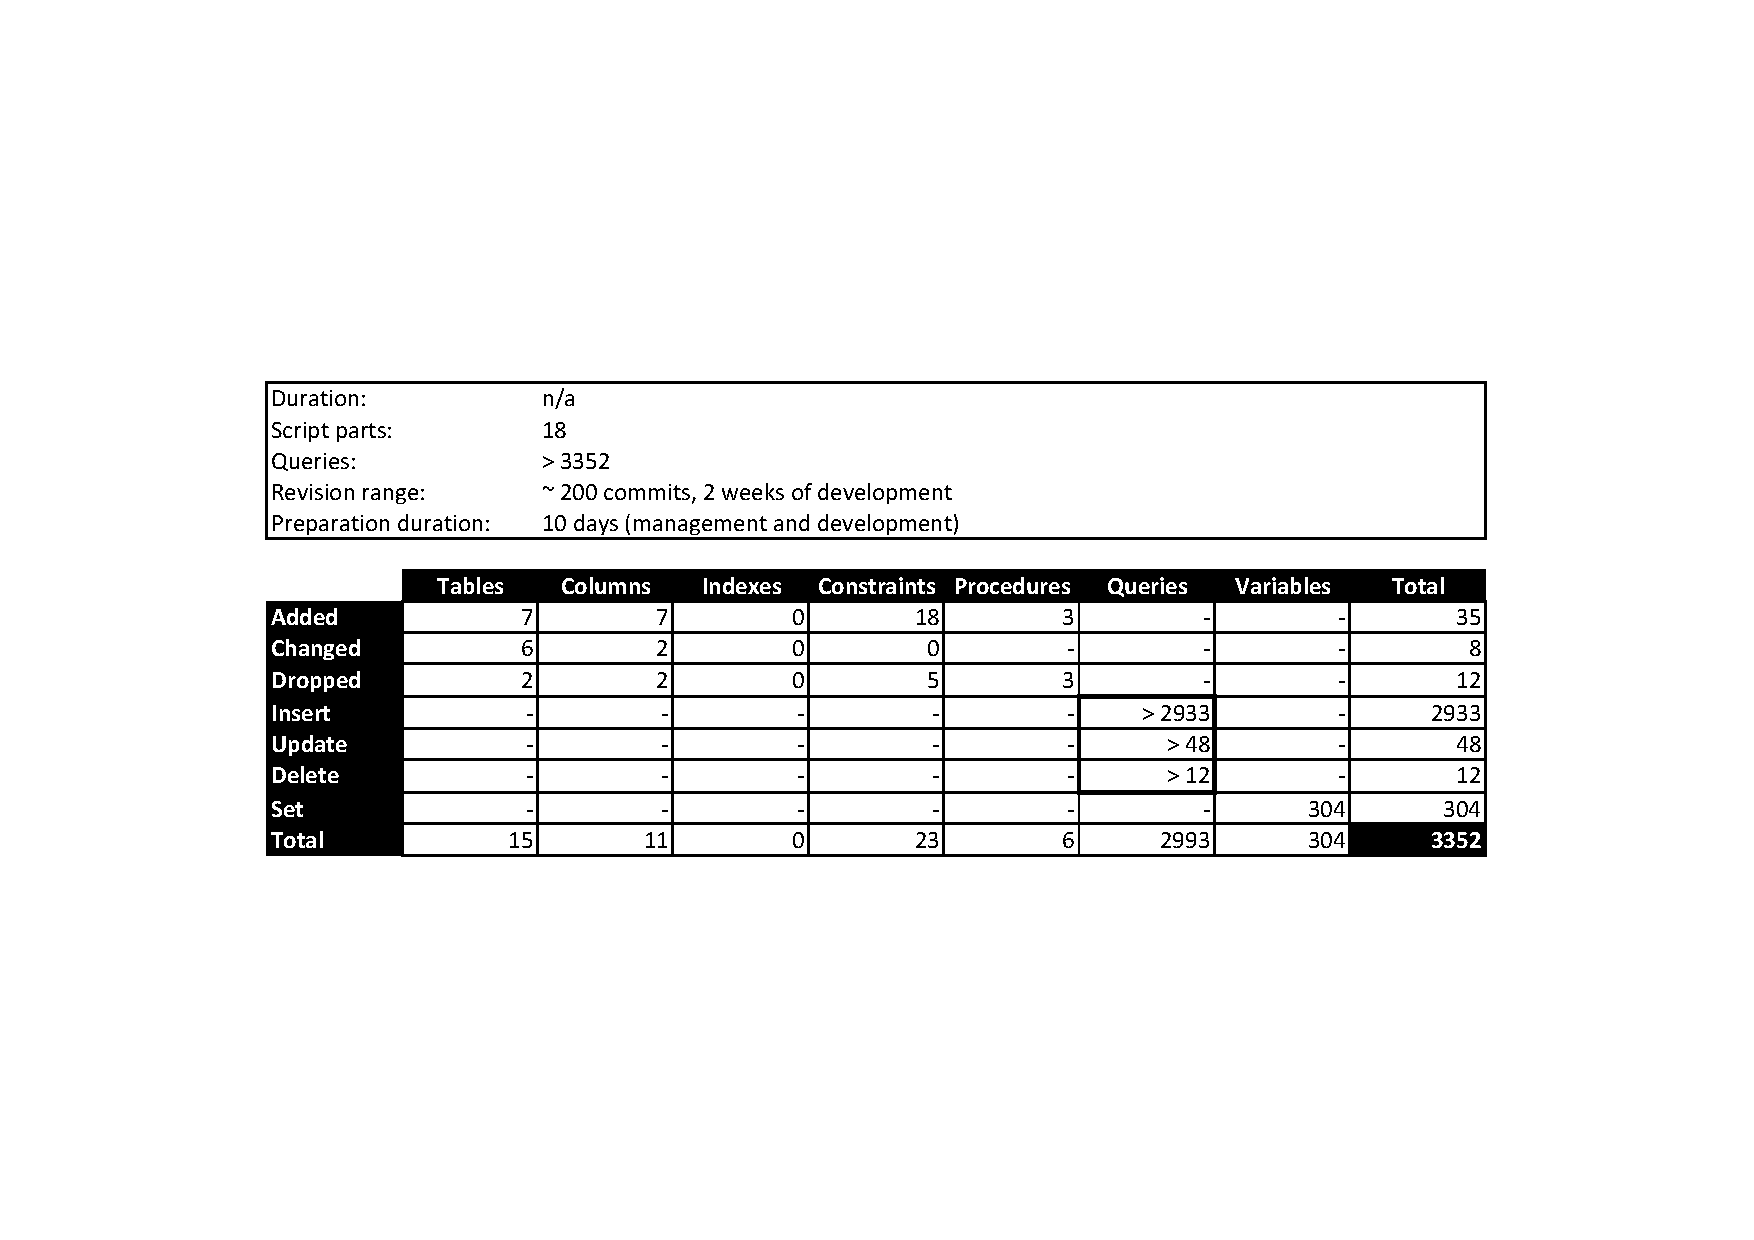
\includegraphics[scale=0.65]{images/Statistics_mig1.pdf}
        \caption{Statistics for a sample migration before introduction of framework}
        \label{fig:StatMig1}
\end{figure}

As we shown on the \autoref{fig:StatMig1}, the statistics are quite interesting. We see that we have run more than 3300 queries. This number is approximative due to the fact we use stored procedures. The methodology to gather the statistics was just to count the statements in the script we run. It means, in the case of stored procedures, that we had count only one time each statement written in the script. It is clearly a naïve approach. We have only the minimum of insert, update and delete queries. We had not monitored the time that the migrations took in our production environment. The way we handle the statistics is clearly a point of improvements. 

The preparation of final scripts were done by hand. It means that each script part was added manually to final scripts. All the preparations took approximatively ten days with a lot of work done by hand. A lot of repetitive tasks that encourage errors and delays. We clearly saw that we needed more structure to handle correctly our migrations. These migrations were quite anarchic.

\subsection{Migration with a basic framework}

For these migrations, we had the time to put in place some concepts, process and tools. We have created a tool to automatize the creation of the final script from the different script parts. It allowed to save time and manual handling. By the way, it drastically reduced the risk of errors and missed scripts. We had introduced a basic process to help the developer to write migration script parts. The process we used for these migrations are shown on \autoref{fig:MigSchemaGenMainPremise} where it is a premise of the actual process we use. Basically, the process is just a formalization of the tasks we instinctively did. At this time, we did not have any documentation that each developer can use to write his scripts. Each developers asked the migration manager to know what and how to do the required tasks to prepare migrations.

The tool we wrote is a script in Ruby\cite{ruby} that checkout the scripts from our subversion repository. Then, the different files that are involved in the migrations are concatenated together in the chronological order. From there, the script allows to use some commands to manually reorder the script parts to get the final sorted script. This script is a previous version of the pseudo code presented in \autoref{sec:buildingScript}. The usage of this tool required a lot of knowledge about the script parts for the correct ordering. We needed to know where to put each file due to the basic algorithm to auto-sort the migration parts.

\begin{figure}[h]
        \centering
        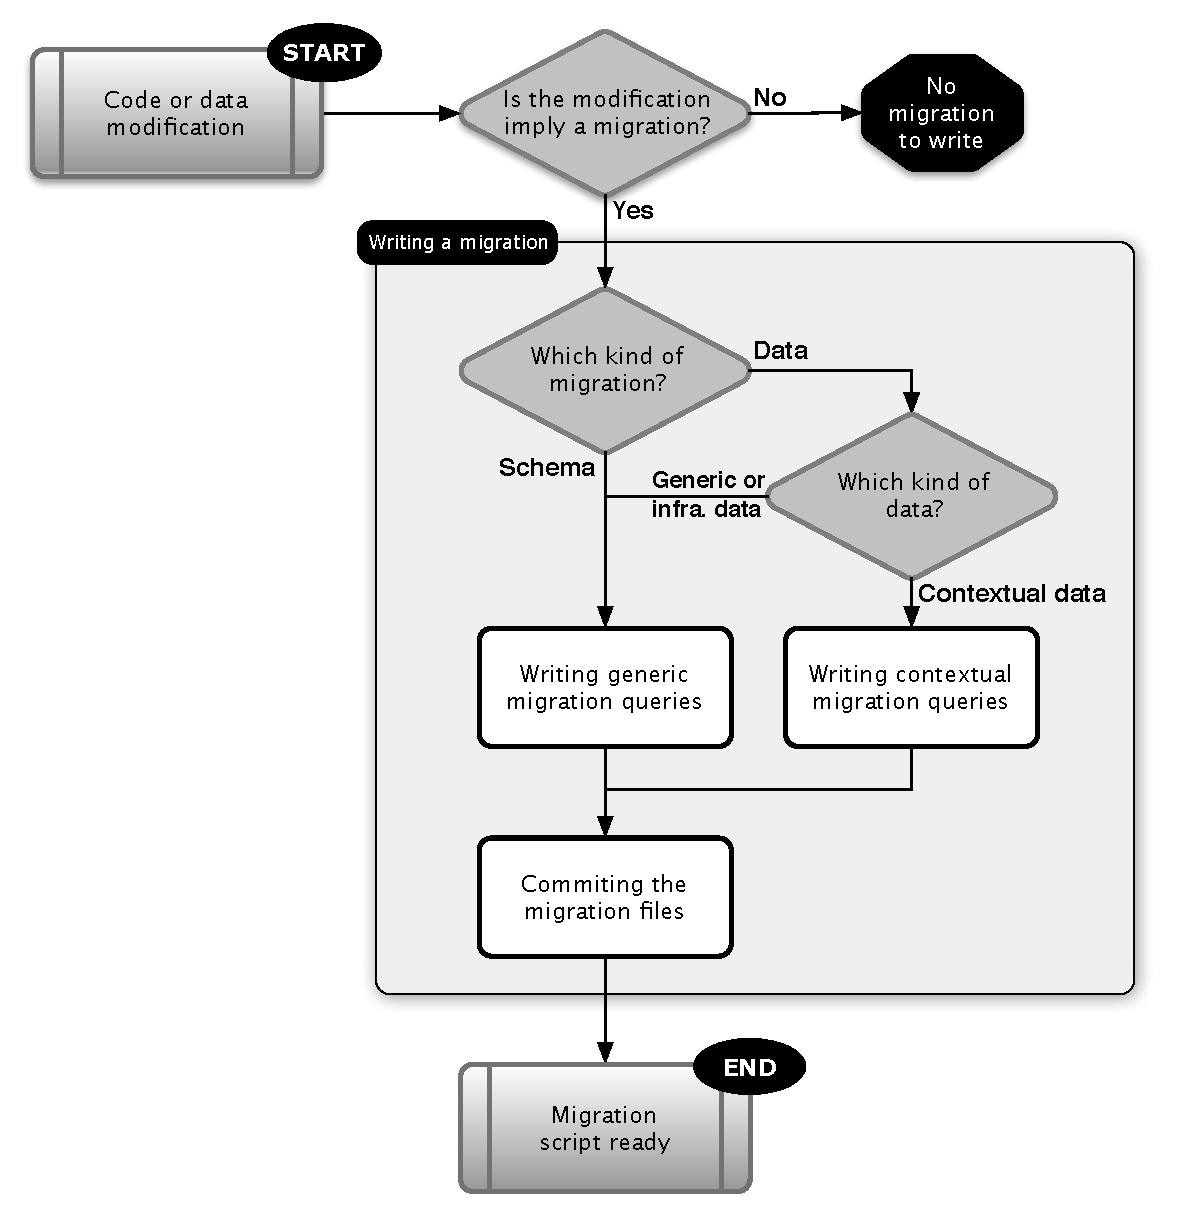
\includegraphics[scale=0.50]{images/mig-schema-gen-main-premise.pdf}
        \caption{Premise migration process}
        \label{fig:MigSchemaGenMainPremise}
\end{figure}

Unfortunately, we were not able to follow regularly the modifications done with an impact of database schema. We accumulate some delays in the monitoring of the modification and in the script writing. We tried to write the scripts each time it was required without success due to the unformalized process. In addition, the rules were not so clear and some mistakes were done in the writing process. Some queries that are contextual were written in generic migration files and vice versa.

\begin{figure}[h]
        \centering
        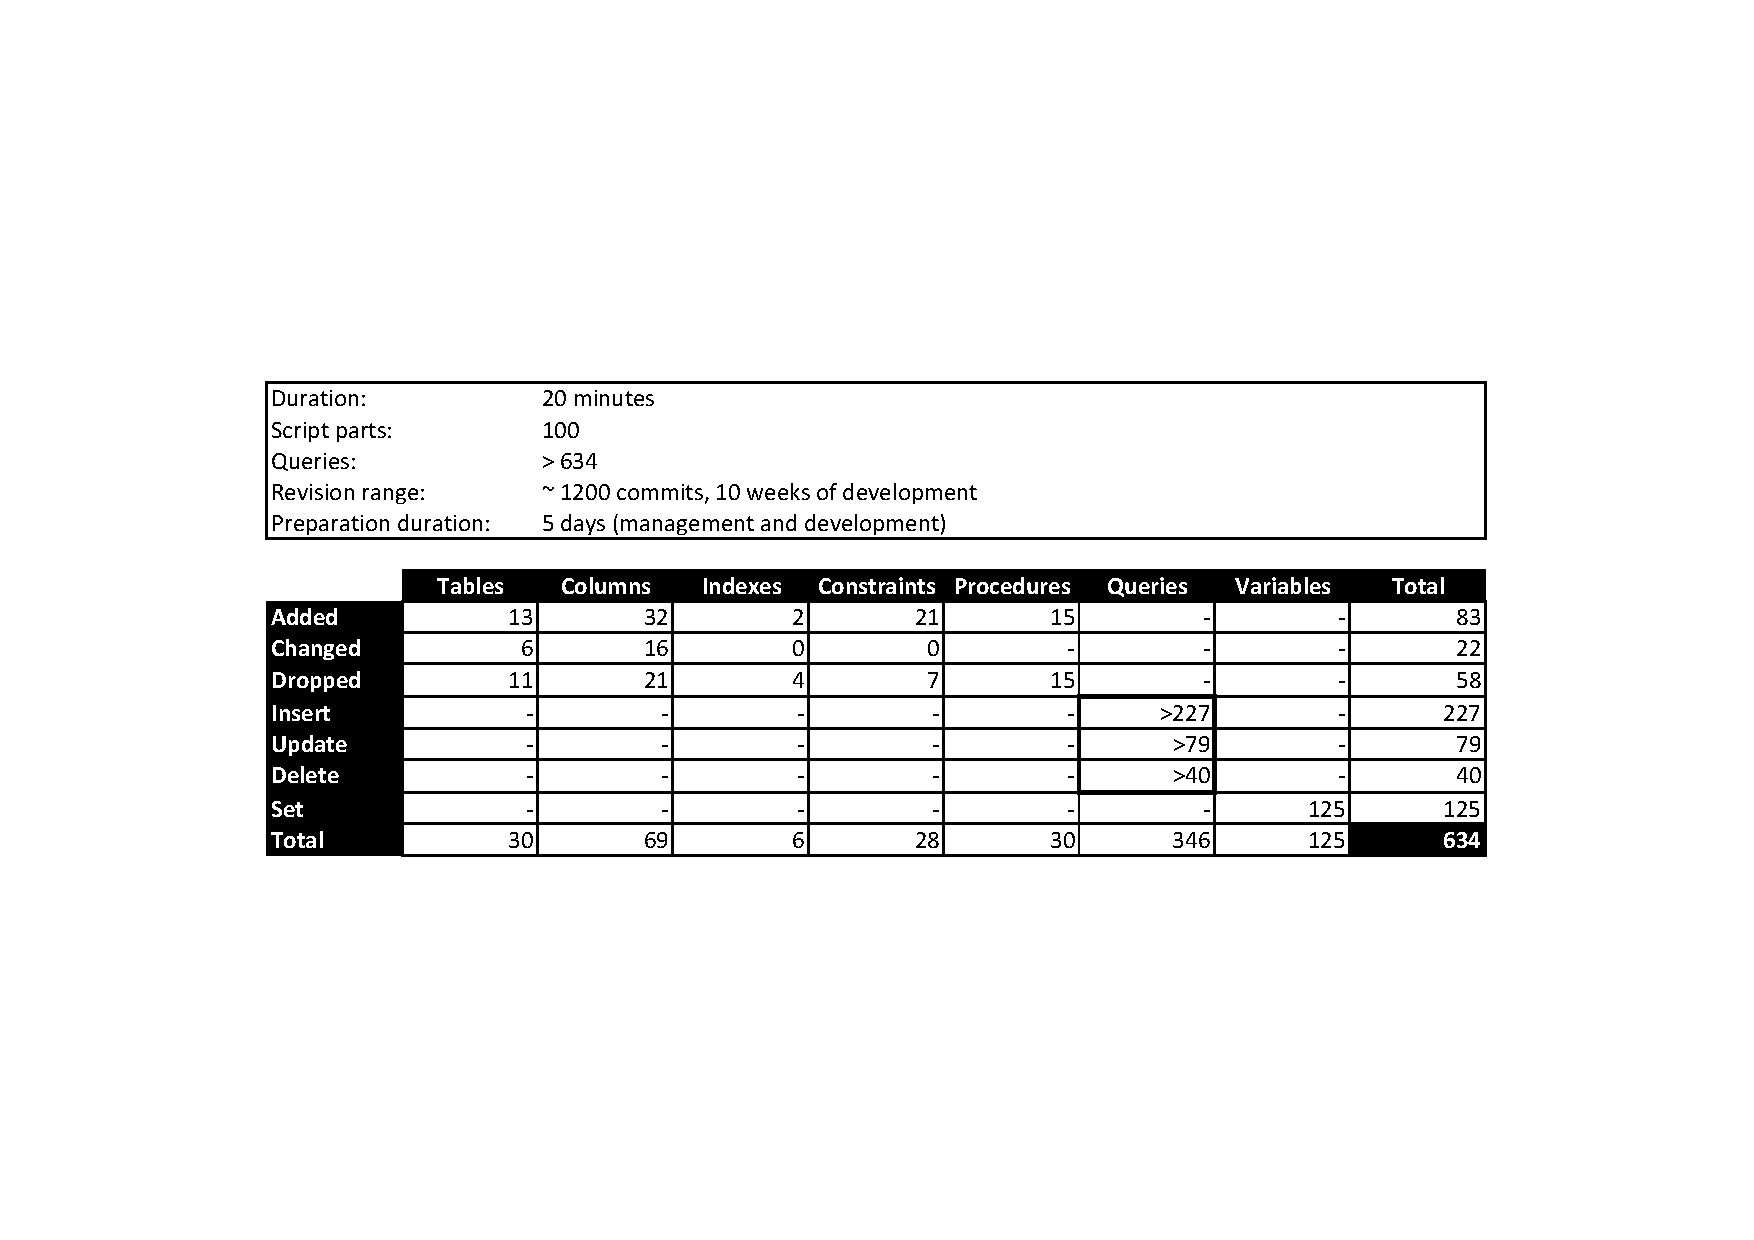
\includegraphics[scale=0.65]{images/Statistics_mig2.pdf}
        \caption{Migrations with a basic process}
        \label{fig:Statistics_mig2}
\end{figure}

Nevertheless, we had reduce the preparation time for a migration. The sample migration on \autoref{fig:Statistics_mig2} shows the growth of commits for a migration with a direct impact of the number of migration script parts. By the way, the statistics were handled in the same way than the previous migrations with count from the migration scripts to. They remain basic and not totally relevant.

\subsection{Migration with an enhanced framework}

At this stage, we had put in place improved rules that the developer team could have access and could use to write the migration script parts. The rules try to cover all the aspects we need. From the previous rules we proposed, we have done some modifications to match the technologies, tools and frameworks. For example, we replaced the numbering rules by revision number usage from the Subversion info. Each commit from repository in Subversion is tagged with a unique revision number that we can use. It allows to know that a migration script part referred to a specific revision that introduced the schema or data change. These changes show that our framework is quite flexible that could be adapted to a specific environment. Aside these changes, the rules remain the same and were used in the state we presented them.

Another improvement we did was the tool. We continued to developed the script building tool with the algorithm we presented in pseudo code \autoref{pcode:buildingScript1} and followings. We also introduced the enrichment of scripts with the queries for automatic metering. From this point, the metrics we gathered are not obtained by hand but directly from the database. As we use MySQL, we have specialized our tool. We use directly database informational schema to gather the metrics. MySQL offers some statistical data like number of queries, number of inserts, number of updates and so on. We manipulate these values to calculate our metrics that we will store directly into the application database tables.

We have also added some tables into the application database schema to keep migration information from time to time. Each migration will populate the additional tables with the metrics values, migration info and so on. We use exactly what we have explained in \autoref{sec:migInfoAndStats}. These information have multiple usage in addition to have interesting data about the data migration. We can follow each migration and from an audit point of view, these data are really useful.

Last but not the least, we have introduced all these new artifacts to the developers. We convinced each developer to follow the rules and why it is important to follow the rules. It was not an easy task due to the fact that each developer has his own habits. It is clearly important that the development team understand the goals to be strict about migration process. They have a major role to play in the process by writing atomic migration part that correspond to any data model changes. We must be able to reproduce at any time any migration from scratch.

\begin{figure}[h]
        \centering
        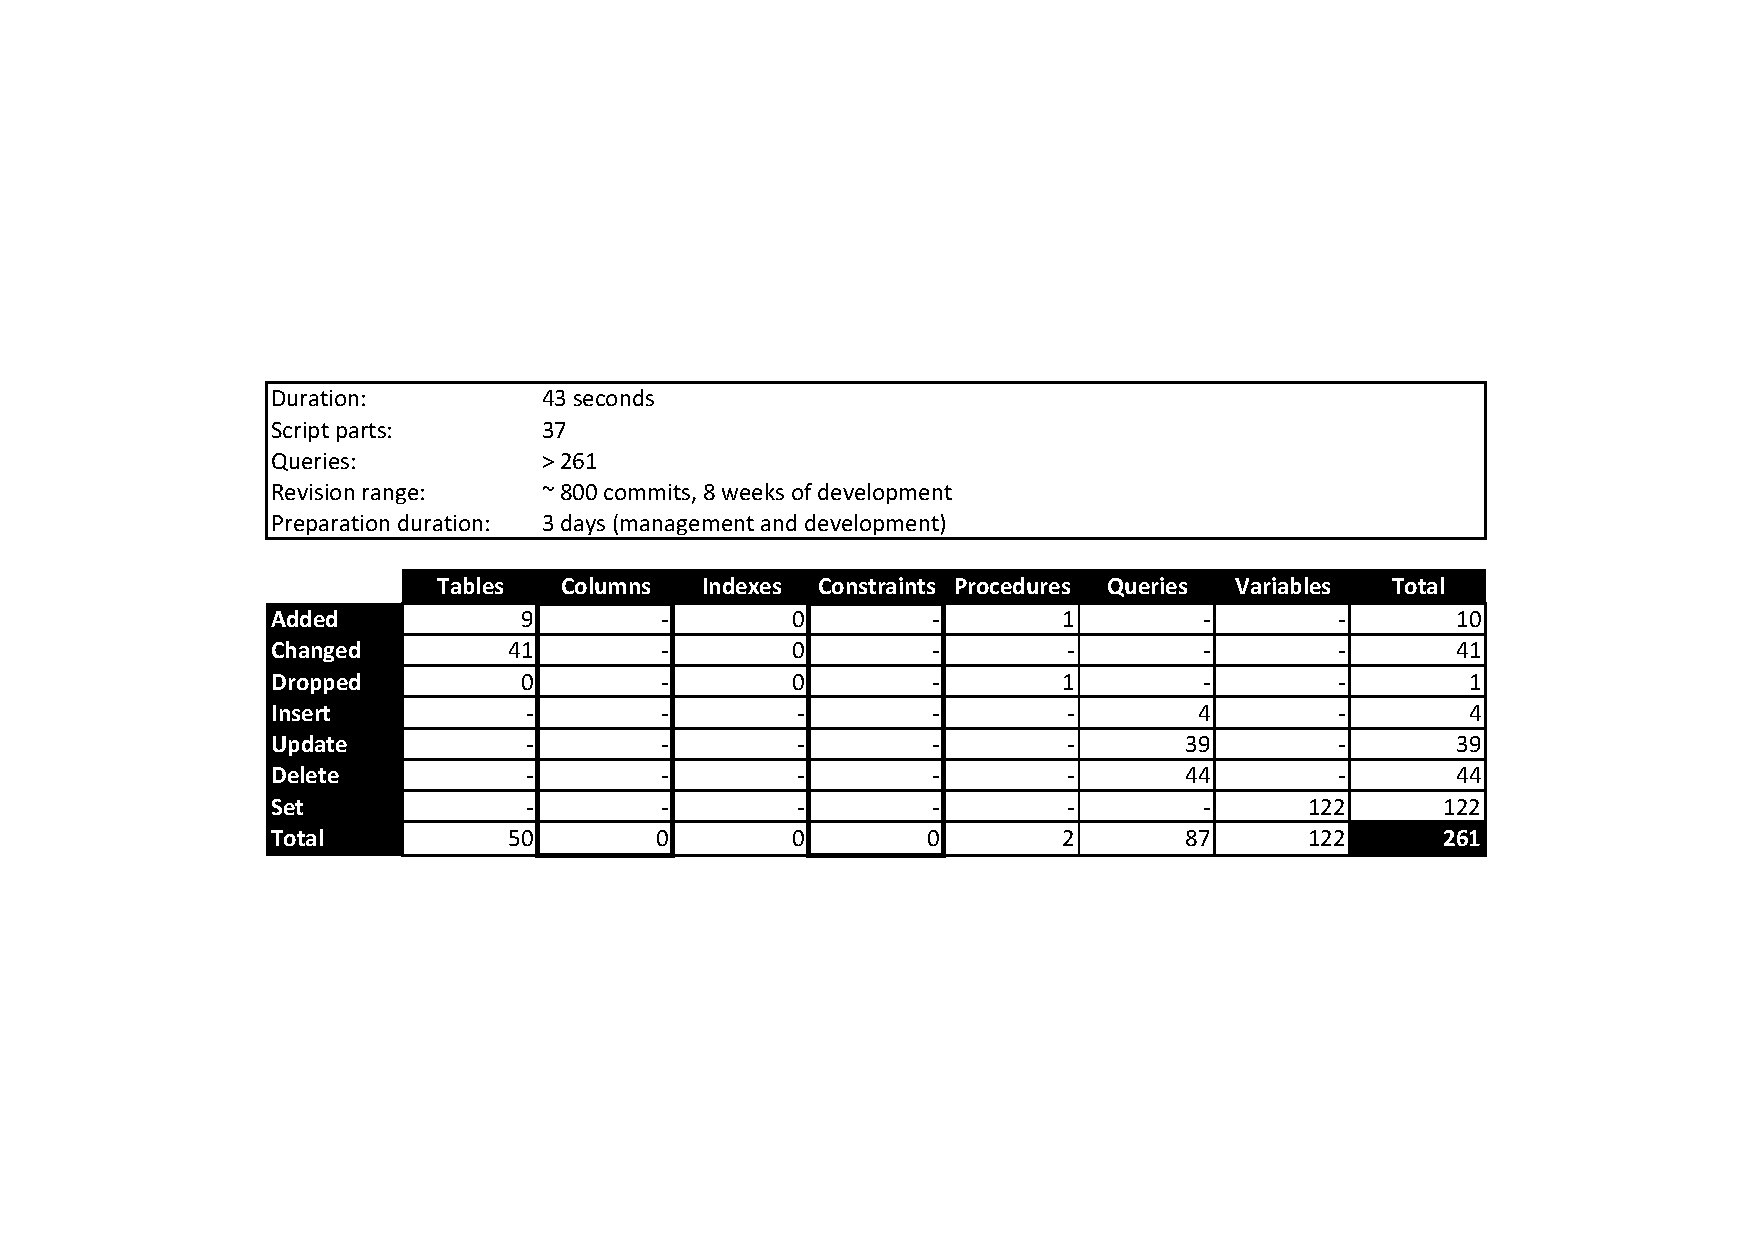
\includegraphics[scale=0.65]{images/Statistics_mig3.pdf}
        \caption{Migration with an enhanced process}
        \label{fig:Statistics_mig3}
\end{figure}

The migration statistics example in \autoref{fig:Statistics_mig3} shows that we can handle migrations with ease. The total of commits remains important but the preparation time was reduced. The time to invest in a migration starts to be reasonable. We can also see that the statistics are quite strange. There are no data for the constraints and columns but the script contains modification for these kind of modifications. We suppose that the metrics that we gather automatically from MySQL are not present directly. We have probably these data confused in other metrics like table modifications. We have to investigate and correct these errors but it is clearly an improvement than doing by hand.

\subsection{Evolution summary}

As we have described, the evolution of our methods to migrate our applications conduct us to develop tools, process and rules. Without these, we clearly loose time and improve the risks of errors. We know that we have a long road to cross to reach a more satisfying situation. We absolutely need robustness and confidence in our migration scripts that we do not have so much actually. We need to think about testing our migrations as soon as possible in the whole process to preventively detect any defect.





